\documentclass{report}                                                           
        
\usepackage{titlesec}
\titleformat{\chapter}
  {\normalfont\LARGE\bfseries}{\thechapter}{1em}{}
\titlespacing*{\chapter}{0pt}{3.5ex plus 1ex minus .2ex}{2.3ex plus .2ex}
\usepackage[left=1in, right=1in, top=1in, bottom=1in]{geometry}
\usepackage{hyperref} 
\usepackage{xcolor} 
\usepackage{ulem}                     
\usepackage{graphicx} 
\usepackage{rotating}
\usepackage{setspace}
\usepackage{longtable}
\usepackage[acronym]{glossaries}
\usepackage[binary-units=true]{siunitx}
\usepackage{multirow}
\usepackage{subcaption}
\usepackage{algorithm}
\usepackage{algorithmicx}
\usepackage{algpseudocode}
\algnewcommand\algorithmicforeach{\textbf{for each}}
\algdef{S}[FOR]{ForEach}[1]{\algorithmicforeach\ #1\ \algorithmicdo}
\algblock{Input}{EndInput}
\algnotext{EndInput}
\algblock{Output}{EndOutput}
\algnotext{EndOutput}
\newcommand{\Desc}[2]{\State \makebox[2em][l]{#1}#2}
                                                                                 
\newcommand{\note}[1]{\textcolor{blue}{\textit{note}: #1}}                       
\newcommand{\tristan}[1]{\textcolor{red}{TG: #1}}                                
\newcommand{\weird}[1]{\uwave{#1}}  

\makeatletter
\newcommand{\setword}[2]{%
  \phantomsection
  #1\def\@currentlabel{\unexpanded{#1}}\label{#2}%
}
\makeatother


\newacronym{hpc}{HPC}{High Performance Computing}
\newacronym{fuse}{FUSE}{Filesystem in User Space}
\newacronym{hdfs}{HDFS}{Hadoop Distributed File System}
\newacronym{ost}{OST}{Object Storage Target}
\newacronym{mdt}{MDT}{Metadata Target}
\newacronym{mds}{MDS}{Metadata Server}
\newglossaryentry{ml}{
    name = $M\_{l}$ ,
  description = The makespan with page cache,
}


% Fix link colors
\hypersetup{
    colorlinks = true,
    linkcolor=red,
    citecolor=red,
    urlcolor=blue,
    linktocpage % so that page numbers are clickable in toc
}
\setcounter{tocdepth}{1}

\makenoidxglossaries
\begin{document} 
    \begin{titlepage}
       \begin{center}

           \hspace{0pt}
                \vfill
                    \textbf{Porting Big Data optimizations to scientific workflows on HPC}
                \vfill
           \hspace{0pt}

           \vspace{2cm}

           \textbf{Valerie Hayot-Sasson}

           \vfill

           ENCS 8011: Graduate Seminar\\

           \vspace{0.8cm}

           Department of Software Engineering and Computer Science\\
           Concordia University\\
           \today

       \end{center}
    \end{titlepage}
    
    \spacing{1.5}
    \begin{abstract}
        With the growing rise in open scientific datasets, there is an increased
        need in efficient data management strategies to offset the transfer-related
        costs that may occur during processing on \gls{hpc}
        environments. Big Data frameworks such as Hadoop MapReduce and Apache 
        Spark have introduced and popularized two major data management strategies:
        Data locality and In-memory computing. Although such frameworks are 
        heavily used in industry, they remain seldom used in imaging analysis 
        pipelines as they are not well-adapted for the processing of such 
        datasets and are not designed to be executed on heterogeneous architecture 
        such as \gls{hpc} clusters. Furthermore, in the case of neuroimaging, our main 
        use case, the processing of data relies on pre-existing command-line tools,
        which would need to be rewritten in order to be adequately written using
        the frameworks. However, we have found that data locality and in-memory
        computing combined can bring up to a 5x speedup to neuroimaging workflows.

        Here we present progress on Sea, a hierarchical filesystem leveraging 
        libc interception to enable optimized data placement strategies for 
        scientific workflows running on \gls{hpc} clusters. Implementation details and
        an evaluation of the designed performance model will be discussed.
        
         
    \end{abstract} 
    %\printglossary[title=List of Symbols]
    \printnoidxglossary[type=\acronymtype,title=List of Abbreviations]
    \tableofcontents

    \chapter{Introduction}

    The cost data transfers rises with the increase in dataset size. While these costs
    have previously been neglected in scientific computing, where applications had
    notoriously been compute intensive, there are becoming a sign
    
    \chapter{Background}
        \section{Big Data optimizations}
            \subsection{Data locality}
            \subsection{In-memory computing}
        \section{Scientific pipeline engines}
        \section{HPC infrastructure}
            \subsection{Architecture}
            \subsection{Scheduling}
            \subsection{Parallel file systems}
            \subsection{Burst buffers}
        \section{The Linux Page Cache}
        \section{User-space file systems}
            \subsection{FUSE}
            \subsection{libc interception}
            \subsection{System call interception}

    \chapter{Evaluation of Big Data optimizations on HPC}\label{chp:eval}

        Before developing any new software for data management, we need to
        determine if the proposed strategies are beneficial to scientific computing.
        Should these strategies be beneficial to scientific computing, we should try
        to develop strategies to better adapt them to \gls{hpc} environments. Furthermore,
        other hardware to improve performance of Big Data applications on \gls{hpc}
        should also be investigated.

        In this section, we will go over three of my published works evaluating existing
        strategies. All of the works mentioned below use the same algorithm tweaked
        slightly, depending on the application, to benchmark
        performance (Algorithm~\ref{alg:incrementation}). Section~\ref{section:ccgrid2019} will provide a summary of my
        paper titled, \textit{Performance Evaluation of Big Data Processing Strategies for Neuroimaging}
        published at CCGrid in 2019. Section~\ref{section:escience2019} will provide
        a summary of my paper titled \textit{Evaluation of pilot jobs for Apache Spark applications on HPC clusters}. We will conclude with my third paper titled,
        \textit{Performance benefits of Intel® Optane™ DC persistent memory for the parallel processing of large neuroimaging data}, in Section~\ref{section:ccgrid2020}.

            \begin{algorithm}\caption{Incrementation}\label{alg:incrementation}
            \begin{algorithmic}[1]
            \Input
            \Desc{$x$}{a sleep delay in seconds}
            \Desc{$n$}{a number of iterations}
            \Desc{$C$}{a set of image chunks}
            \Desc{$fs$}{filesystem to write to (mem, tmpfs, local disk, Lustre).}
            \EndInput
            \ForEach{$chunk \in C$}
            \State read $chunk$ from Lustre
            \For{$i \in [1, n]$}
                \State $chunk\gets chunk+1$
                \State sleep $x$
                \If{$i < n$}
                \State save $chunk$ to $fs$
                \EndIf
            \EndFor
            \State save $chunk$ to Lustre
            \EndFor
        \end{algorithmic}
        \end{algorithm}
        
        \section{Evaluation of data locality and in-memory computing}\label{section:ccgrid2019}

        Big Data strategies, such as data locality and in-memory computing, have been shown 
        to provide significant speedups to large text-processing applications, however,
        their use in scientific communities, such as neuroimaging, remain limited. 
        Although there has been some research done to show the benefit of utilizing
        Big Data frameworks for scientific computing, many of the popular scientific
        pipeline engines lack implementation of these strategies. The aim of this paper
        was to investigate the performance improvements that could be gained
        from the use of data locality and in-memory computing for scientific application 
        and design a model that described when a performance improvement could be expected.
        

        Our model to describe when Big Data strategies would be useful is described in
        Equation~\ref{eq:bd}. Essentially, when there is a sufficient amount of data ($D$)
        being generated given the total application compute time ($C$) such that the disk
        bandwidth ($\delta$) could not support all the I/O given the number of
        application parallel threads ($\gamma$), it is useful to leverage Big Data strategies.
        Any disk writes below the threshold is expected to be able to leverage page cache.


        \begin{equation}\label{eq:bd}
            \frac{D}{C} \le \frac{\delta}{\gamma}
        \end{equation}

        To evaluate the designed model, we created both and Apache Spark and 
        Nipype application using
        Algorithm~\ref{alg:incrementation} and applied in on a \SI{13}{\mega\byte}
        T1W image from OpenNeuro~\cite{openneuro} and the partial
        and full \SI{76}{\gibi\byte}{BigBrain} image. All experiments were conducted
        on Dell EMC's Zenith cluster~\cite{zenith} using node-local tmpfs, SSD,
        and their Lustre server for storage.

        For our experiments, we varied the number of iterations (1, 10, 100),
        sleep time (2.4, 3.44, 7.68, 320s), number of blocks (30, 125, 750) and
        file size (\SI{13}{\mega\byte}, \SI{38}{\gibi\byte}, \SI{76}{\gibi\byte}).
        
        As confirmed by the model, when increasing the amount of application intermediate
        data produced (increasing the number of iterations), Big Data strategies
        can play a great role in improving application performance. Lustre was
        found to be 3.82~x slower than Spark in-memory at 100 iterations, whereas it
        was was 2.67~x slower at 10 iterations. Conversely, increasing task duration
        meant a decreased speedup. Lustre was 1.01~x slower than Spark in-memory
        at 320s tasks, whereas it was 3.25~x slower with 2.4 second tasks.

        Lustre's performance remained worse than that of in-memory and SSD in the
        experiments in which we varied the number of files and file size. Lustre's
        performance was only comparable for the \SI{13}{\mega\byte} image.

        Overall, it was found that data locality alone (writing to node-local storage)
        could bring a 3.2~x speedup,
        whereas in-memory alone could bring up to a 1.6~x speedup. Data locality and
        in-memory computing combined was found to bring up to a 5.3~x speedup.
        It was thus concluded that data locality plays a more significant role in
        improving application makespan.


        \section{Pilot scheduling for Spark on HPC}\label{section:escience2019}

        \gls{hpc} clusters typically rely on batch provisioning schedulers (e.g. SLURM, PBS)
        to allocate resources. When a user requests a resource allocation, their jobs
        are placed in a priority queue based on previous cluster usage, current resource
        requirements and overall node availability. For typical \gls{hpc} applications,
        this is not a problem. However, Big Data applications would rely on significant
        amounts of resource requirements and may end up waiting on the resource allocation
        queue for a significant amount of time. In this case, pilot scheduling, which
        would enable dynamic provisioning of Spark clusters on \gls{hpc} may significantly
        reduce batch scheduler queue time. In this paper, we designed and implemented
        a library called \texttt{Spa} that would streamline the dynamic provisioning of
        Spark clusters on \gls{hpc} infrastructure and evaluated the makespan differences
        (including queueing time) between typical batch provisioning and 
        dynamic pilot provisioning. In addition we devised a model to
        describe the relation between makespan and number of pilots.

        \begin{equation}\label{eq:makespan}                                                       
            \frac{M_{batch}}{M_{pilot}} = \frac{W_{pilot}}{W_{batch}}
        \end{equation} 
        As per Equation~\ref{eq:makespan}, the ratio between the makespan ($M$) of batch
        and pilot provisioning should be the same as the ratio between the average number
        of Spark workers active ($W$), where the average number of where the average number
        of Spark workers can be defined as:
        \begin{equation}\label{eq:avgw}
            W = \frac{1}{M}\int_0^M{w(t)dt}
        \end{equation}

        To evaluate the two strategies, we used two Compute Canada \gls{hpc} clusters: 
        Cedar and B\'eluga. The pilot scheduler was configured to generate either 8 or 16 pilots.
        Batch, in contrast, consisted of a single resource request containing all
        required application resources.

       We performed a total of four experiments, each with an increasing number of nodes required.
       Each node was equipped with 112~GB of RAM, a single CPU per task, 16 tasks/node
       and a wall time of 2h30. For each configuration, we increased the number
       of nodes used by 1. Task delay was also increased with the increasing number
       of nodes. At 1 node, task delay was set to be 45s. It varied
        between 90, 120 and 180 with each additional node.


        Our results found that there is little advantage in using pilot 
        jobs as the queueing time between batch and pilot provisioning 
        remained similar. However, this could be an indication that not enough 
        resources were requested. We expect that  as the number of resources 
        increase, pilot provisioning may begin to out-perform batch provisioning.

        \section{Intel Optane storage for scientific computing}\label{section:ccgrid2020}


        While there have been software advances to the reduction of data transfer times
        on \gls{hpc} systems, there have also been hardware advances. One of such 
        hardware advances is the Intel Optane DC Persistent Memory, which is a 
        cost-effective solution to increasing available memory for use with Big Data
        applications. In this paper, we evaluate the effectiveness of using
        Intel Optane DC Persistent Memory for Big Data scientific applications.
        We additionally compared Memory Mode to App Direct Mode to determine which
        mode provides better performance for a given application.
        
        For our experiments, we utilized a server containing 12 \SI{64}{\giga\byte} 
        DRAM devices (total
        \SI{768}{\giga\byte}), 12 \SI{256}{\giga\byte} Intel Optane DC devices (total:
        \SI{3}{\tera\byte}), a single \SI{240}{\giga\byte} SSD and access to
        a shared Isilon cluster, consisting of 5 nodes each containing 36 hard disk drives.
        With the exception of the SSD, none of the devices were configured to use memory
        as a writeback cache when persistently storing data.


        Given that it is assumed that the storage devices will only perform sequential
        I/O, the makespan ($M$) is expected to be greater or equal to the amount of time it
        takes to read and write all the data (Equation~\ref{eq:optane}).
        The amount of time it takes to  
        it takes to read and write the data can be summarize as the total data read
        and written over their respective bandwidths: $R$ and $W$.

        \begin{equation}\label{eq:optane}
            M \ge \frac{D}{R} + \frac{D}{W}
        \end{equation}

         To evaluate Intel Optane DC Persistent memory, we applied 
         Algorithm~\ref{alg:incrementation} on the \SI{76}{\giga\byte} 40~$\mu$ and 603GB
        20~$\mu$ BigBrain, in addition to a real neuroimaging pipeline (\href{https://github.com/BIDS-Apps/example}{BIDS App
        Example}), on the entire CoRR
        dataset~\cite{corr}. There were 125 614~MB blocks for the
        40~$\mu$ and 1000 617~MB for the 20~$\mu$ BigBrain.  The BIDS App
        Example consisted of the execution of a brain extraction application on
        only the anatomical (T1W) images of the dataset, operating only on a
        reduced portion of the dataset. Each experiment was
        executed 3~x in both Memory Mode and App Direct Mode. To evaluate
        scalability of the storage devices, 25 and 96 parallel processes were
        used.

        With the exception of DRAM, Optane was found to perform significantly
        better than alternative storage devices when applied to large neuroimaging
        datasets. When Memory Mode and App Direct mode were compared to each other,
        Memory Mode appeared to be faster. This is likely due to the fact that App
        Direct mode does not leverage any writeback cache. It is believed that Memory
        Mode could significantly improve the speeds of data visualization, whereas App
        Direct could greatly improve the runtime of Big Data scientific applications
        by being leveraged as a burst buffer.



    \chapter{The Sea filesystem}
    \section{Introduction}
    In previous chapters, we discussed that while data-intensive scientific 
    applications may gain significant speedups from leveraging Big Data optimizations,
    they must be reimplemented for use with Big Data frameworks. Furthermore, Big Data
    frameworks are not well suited for execution on \gls{hpc} systems where the 
    communication between workers can only be achieved through the use of overlay
    clusters.

    We have also addressed alternative ways to obtain data-related performance speedups on \gls{hpc}
    using either burst buffers, Optane technology or Big Data filesystems such as \gls{hdfs}
    or Alluxio. While these solutions do reduce the cost of data transfers, they incur
    a learning overhead for users and may require the purchasing of additional infrastructure and
    adoption by system administrators.

    In addition to existing solutions, there is a third alternative to bringing data
    locality and in-memory computing to scientific applications running on \gls{hpc}
    without requiring system administrator intervention nor the reinstrumentation
    of existing scientific applications. This may come in the form of a user-space 
    on-the-fly tiered file system. In this chapter we introduce Sea, a volatile user-space file
    system that can leverage all available storage on a given compute node with the aim
    of enabling data locality and in-memory computing for scientific workloads.

    The goals of Sea are as follows:
    \spacing{0.5}
    \begin{enumerate}
            \item make efficient use of available storage devices to minimize data
                transfer costs
            \item adapt to changes in storage bandwidth due to device use
            \item exist entirely in user space
            \item function without application reinstrumentation
            \item Exist exclusively for the duration of a single application
    \end{enumerate}

    \note{mention that the code is open-source, provide link, etc}
    \spacing{1.5}
   Sea will enable users to leverage its performance optimizations without intervention
   from system administrators nor specific understanding of the underlying infrastructure.
   In this chapter we will discuss the ongoing work that has been put into the development
   of Sea. Section~\ref{design} will present the design decisions that went into the
   implementation of Sea. In Section~\ref{model}, we will go over a Lustre and Sea
   performance model that should describe the upper and lower bounds of performance by using
   the default (Lustre) method and Sea. Section~\ref{exp} will describe the experiments that we
   used to evaluate our models and Sea. We will then report the results of our evaluation
   in Section~\ref{results} and conclude with a discussion in Section~\ref{discussion}.
    
   \section{Design}\label{design}
   Sea aims to provide speedups to scientific applications running on \gls{hpc}
   by redirecting application intermediate data to compute-local storage (e.g. tmpfs,
   SSD, HDD), whenever possible.
   To do so effectively, it must make sure to do so with a minimal overhead, such as
   to not render accesses to local storage slower than that of the underlying parallel
   file system. Furthermore, Sea should be careful not to reduce the performance of the
   underlying file system.

   With scientific applications, it is sometimes necessary to maintain copies of
   the intermediate data. Traditional Big Data engines do not invest in maintaining
   the intermediate data on permanent storage as the belief is that it is generally 
   more costly to store the data than to recompute it at a later time. Nevertheless,
   they do provide the ability to persist data to disk, particularly when the 
   costs of recomputation outweigh that of storing the data. Even if scientific application
   tasks could easily be recomputed, some tasks leverage randomization which would make
   it difficult to reproduce with recomputation unless the seed was fixed. Therefore,
   Sea must enable users the ability to materialize all necessary data to the parallel
   file system without incurring significant overheads during transfer to slower storage.

   \note{talk about the design\ldots mountpoint etc}

   In this section, we will discuss the design that went into Sea.
   Subsection~\ref{subs:assumption} will discuss the assumptions that were made
   when developing Sea. Subsection~\ref{subs:libcintersection} will look at how
   Sea intercepts calls and redirects them through the appropriate file system.
   Subsection~\ref{subs:configuration} will describe what type of user input
   is required to ensure proper functioning of Sea and Subsection~\ref{subs:flushandevict}
   will look at how flushing and eviction is approached by Sea.

   \subsection{Assumptions}\label{subs:assumption}

   Sea makes certain assumptions in order to achieve proper functioning. For Sea to
   work at all, it must be used in a Linux environment. Since most \gls{hpc} clusters
   use Linux distributions, it is not believed to be a major limitation of Sea. We test
   the proper functioning of Sea over various Linux distributions through continuous
   integration. Sea is currently compatible for use with Centos 6 through 8, Fedora 32
   and Ubuntu Xenial and Bionic.

   Since Sea leverages libc interception to intercept file system calls, we must
   make the assumption that the selected scientific application uses the libc library
   to interact with the file system. Additionally, for libc interception to work,
   the application must be dynamically-linked. While this may be problematic in some
   scenarios, we expect that Sea will function for the majority of scientific applications.

    Given that the input data must be read from the parallel file system and the
    output data must be written to the same file system for later access, it is
    not expected that Sea will provide any runtime reduction in scientific applications
    with no intermediate data. Therefore, we make the assumption that significant
    intermediate data will be generated by the application.

    For cases in which all application outputs must be stored to the parallel file
    system, we estimate that the maximum speedup obtained will be the difference in
    compute time. That is to say, given that there is not reduction in I/O to Lustre,
    all we can gain from using Sea is asynchronous writes to Lustre occurring during
    application compute.

   \subsection{libc interception}\label{subs:libcintersection}

   Due to the inherent overheads associated with using user-space file systems and
   performing system call interception, we have decided to leverage libc interception
   for Sea. Adapting the passthrough used in Xtreemfs, we intercept over 100 libc functions.
   The libc functions intercepted by Sea are those that either accept as input a path
   or a pointer to a path.

   After intercepting the call, Sea must determine if the path provided is within the
   Sea mount point. If so, Sea needs to determine the actual location of the file 
   that is being referenced. If a file needs to be created, Sea will travel
   down the storage hierarchy to determine the most efficient filesystem with sufficient
   available space to write to. Filesystems of the same storage layer are randomized in
   order to enable parallel file creation to the same storage layer in the event
   that application tasks need to create files concurrently. If a file already
   exists and needs to be accesses, Sea will traverse through
   the hierarchy looking for the actual path to the file. Directories are created
   in all filesystems existing within Sea's hierarchy. This ensures that there are
   no issues directories have their contents spread out across multiple storage devices.
   Once the actual path of the file is obtained, Sea invokes the intended libc
   function with the actual path.

   \subsection{Configuration}\label{subs:configuration}
   Users must specify their desired configuration in a \texttt{ini} file for the
   proper functioning of Sea. Theses configuration parameters consist of 1) the
   mount point, 2) the number of storage layers and their paths, 3) the log level and
   the logfile path, and 4) the maximum size of a file created by the application and
   the maximum number of concurrent threads.


   The mountpoint is the point of entry for users to communicate with Sea. Outside of
   the mountpoint, the libc calls are still intercepted by Sea, but redirected without
   any path alteration to the libc function. Anything path within the mountpoint 
   must be converted to its actual path before forwarding the call to libc.


   The storage layers each indicate a performance level within the hierarchy. For
   instance, at the top-level, one might consider to place tmpfs devices. In another level,
   local SSDs can be found, with local HDDs in a third, slower level. We expect that the
   final level will typically be a network-based parallel file system, as would be the case
   on \gls{hpc}, however, any kind of file system can be placed there. It is just important
   to note that there can be only a single file system in the last layer, and in the event
   of flushing and eviction, all application outputs will be written to that file system.
   For all other storage layers, multiple filesystems can be specified in the same
   layer using a comma separated list.

   Sea provides five different levels of logging (\texttt{debug}, \texttt{info},
   \texttt{warning}, \texttt{error} and \texttt{none}).
   Logging can occur in the foreground or be saved to a file. Due to the sheer number
   of times libc functions can be called, particularly withing a data intensive workflow,
   it is generally preferable to limit the amount of logging (e.g. \texttt{error} or
   \texttt{none}) to not impede Sea's performance.


   Sea leverage the maximum application file size and number of concurrent threads
   to determine the amount of space required on a filesystem before selecting it for
   a write. In other words, if there is insufficient space on a filesystem for
   $n$ concurrent threads to each write a file of size $x$, this system will not be
   selected for the write. We have selected this approach over the use of locks 
   limit the overheads of Sea.
   \subsection{Flushing and Eviction}\label{subs:flushandevict}

   Files to be flushed and/or evicted to the final storage layer can be specified
   by the user. This is accomplished to populating the \texttt{.sea\_flushlist} and
   \texttt{.sea\_evictlist} files. Both of these files can be populated using relative
   Sea paths containing regex. Paths located in both the \texttt{.sea\_flushlist}
   and \texttt{.sea\_evictlist} files will be asynchronously flushed to the destination
   filesystem and evicted from its current filesystem. Essentially, it is a move operation.
   Files existing solely in the \texttt{.sea\_flushlist} will be flushed to the destination
   filesystem (i.e. a copy operation) whereas files only existing in the \texttt{.sea\_evictlist}
   file will be removed from their current file system. Files that are mentioned in neither
   of the lists will remain in place.

   All flushing and eviction occurs entirely within a separate process. This process
   enables Sea to flush and evict asynchronously, without any major interference
   to the application execution.
   
    \section{The Sea and Lustre model}\label{model}

    \begin{table}
    \centering
    \begin{tabular}{|p{0.03\linewidth}|p{0.7\linewidth}|p{0.2\linewidth}|} 
     \hline
     \multicolumn{3}{|c|}{Makespans} \\
     \hline
     $M_{n}$ & Application I/O to a specific integer level ($n$) of storage device makespan & Eq.~\ref{eq:sea}\\
     $M_{l}$ & Application I/O to Lustre without page cache makespan & Eq.~\ref{eq:lustrenpc}\\
     $M_{c}$ & Application I/O to page cache duration & Eq.~\ref{eq:cache}, \ref{eq:lustrepc}, \ref{eq:sea}\\
     $M_{lc}$ & Application I/O to Lustre including page cache makespan & Eq.~\ref{eq:lustrepc}\\
     $M_{s}$ & Application I/O to Sea without page cache makespan & Eq.~\ref{eq:sea}\\ 
     $M_{sl}$ & Application I/O to the Lustre component of Sea makespan & Eq.~\ref{eq:snc}, \ref{eq:msl} \\
     $M_{sd}$ & Application I/O to the local disk component of Sea makespan& Eq.~\ref{eq:snc}, \ref{eq:msd} \\
     $M_{st}$ & Application I/O to the tmpfs component of Sea makespan & Eq.~\ref{eq:snc}, \ref{eq:mst} \\
     $M_{sc}$ & Application I/O to Sea with page cache makespan & Eq.~\ref{eq:msc} \\ 
     \hline
     \multicolumn{3}{|c|}{Data size} \\
     \hline
     $D_{r}$ & Amount of data read & Eq.~\ref{eq:lustrenpc}\\
     $D_{w}$ & Amount of data written & Eq.~\ref{eq:lustrenpc}\\
     $D_{cr}$ & Amount of data read from cache & Eq.~\ref{eq:cache}\\
     $D_{cw}$ & Amount of data written to cache & Eq.~\ref{eq:cache}\\
     $D_{I}$ & Input dataset size & Eq.~\ref{eq:lustrepc}, \ref{eq:sea}\\
     $D_{tr}$ & Amount of data read from the tmpfs component of Sea & Eq.~\ref{eq:mst}, \ref{eq:dtr}, \ref{eq:ddr}, \ref{eq:dlr} \\
     $D_{tw}$ & Amount of data written to the tmpfs component of Sea & Eq.~\ref{eq:mst}, \ref{eq:dtw}, \ref{eq:ddw}, \ref{eq:dlw} \\
     $D_{dr}$ & Amount of data read from the local disk component of Sea & Eq.~\ref{eq:msd}, \ref{eq:ddr}, \ref{eq:dlr} \\
     $D_{dw}$ & Amount of data written to the local disk component of Sea & Eq.~\ref{eq:msd}, \ref{eq:ddw}, \ref{eq:dlw} \\
     $D_{lr}$ & Amount of output data read from the Lustre component of Sea & Eq.~\ref{eq:msl}, \ref{eq:dlr} \\
     $D_{lw}$ & Amount of output data written to the Lustre component of Sea & Eq.~\ref{eq:msl}, \ref{eq:dlw} \\
     $D_{m}$ & Amount of intermediate data created by the application & Eq.~\ref{eq:dtr}, \ref{eq:dtw}, \ref{eq:ddr}, \ref{eq:ddw}, \ref{eq:dlr}, \ref{eq:dlw}, \ref{eq:msc} \\
     $D_{f}$ & Amount of final output data generated by the application & Eq.~\ref{eq:dtw}, \ref{eq:ddw}, \ref{eq:dlw} \\ 
     $F$ & File size & Eq.~\ref{eq:dtr}, \ref{eq:dtw}, \ref{eq:ddr}, \ref{eq:ddw}\\
     \hline
     \multicolumn{3}{|c|}{Bandwidths} \\
     \hline
     $B_{lr}$ & Perceived Lustre read bandwidth & Eq.~\ref{eq:lustrenpc}, \ref{eq:blr}, \ref{eq:lustrepc}, \ref{eq:sea}, \ref{eq:msl}, \ref{eq:msc}\\
     $B_{lw}$ & Perceived Lustre write bandwidth & Eq.~\ref{eq:lustrenpc}, \ref{eq:blw}, \ref{eq:msl}\\
     $B_{n}$ & Network bandwidth & Eq.~\ref{eq:blr}, \ref{eq:blw}\\
     $B_{or}$ & Lustre \gls{ost} read bandwidth & Eq.~\ref{eq:blr}, \ref{eq:blw}\\
     $B_{ow}$ & Lustre \gls{ost} write bandwidth & Eq.~\ref{eq:blr}, \ref{eq:blw}\\
     $B_{mr}$ & Memory read bandwidth (same as for tmpfs) & Eq.\ref{eq:cache}, \ref{eq:mst}, \ref{eq:msc}\\
     $B_{mw}$ & Memory write bandwidth (same as for tmpfs) & Eq.~\ref{eq:cache}, \ref{eq:mst}, \ref{eq:msc}\\
     $B_{dr}$ & Local disk read bandwidth & Eq.~\ref{eq:msd}\\
     $B_{dw}$ & Local disk write bandwidth & Eq.~\ref{eq:msd}\\
     \hline
     \multicolumn{3}{|c|}{Nodes} \\
     \hline
     $N_{c}$ & Number of compute nodes & Eq.~\ref{eq:blr}, \ref{eq:blw}, \ref{eq:cache}, \ref{eq:mst}, \ref{eq:dtr}, \ref{eq:dtw}, \ref{eq:msd}, \ref{eq:ddr}, \ref{eq:ddw}, \ref{eq:msc}\\
     $N_{d}$ & Number of data nodes & Eq.~\ref{eq:blr}, \ref{eq:blw}\\
     $N_{t}$ & Number of threads per compute node & Eq.~\ref{eq:blr}, \ref{eq:blw}, \ref{eq:dtr}, \ref{eq:dtw}, \ref{eq:ddr}, \ref{eq:ddw}\\
     \hline
     \multicolumn{3}{|c|}{Storage} \\
     \hline
     $O$ & Number of Lustre OSTs & Eq.~\ref{eq:blr}, \ref{eq:blw}\\
     $d$ & Number of local disks & Eq.~\ref{eq:ddr}, \ref{eq:ddw}\\
     $S_{t}$ & Amount of available storage on tmpfs & Eq.~\ref{eq:dtr}, \ref{eq:dtw} \\
     $S_{d}$ & Amount of available storage on local disk & Eq.~\ref{eq:ddr}, \ref{eq:ddw} \\
     \hline
    \end{tabular}
    \caption{Lustre and Sea model symbols}
    \label{table:1}
    \end{table}

    To effectively be able to predict in which scenarios Sea will provide speedup
    over the baseline solution, we require a model. Since different parallel file
    systems may operate differently, our baseline model will be based on Lustre which
    is commonly used on \gls{hpc} infrastructure.

    For our data intensive use cases, the makespan models for both Lustre and Sea can be broken
    down into two components: The amount of time it takes read the data and the amount
    of time it takes to write the data. With more heterogeneous applications (some components 
    are compute intensive whereas others are data intensive), a third component, comprising
    of compute time, can be added. Furthermore, latency make also play a significant role
    application makespan, particularly in scenarios with large amounts of small files.
    We choose to ignore latency costs in our model and make the assumption that the
    application bottleneck is the bandwidth, however, for more accurate estimates we
    might consider the addition of file system latency, as a fourth model component.

    A simplified version of the Lustre makespan model can be defined as follows:

    \begin{equation}\label{eq:lustrenpc}
        M_{l} =  \frac{D_{r}}{B_{lr}} + \frac{D_{w}}{B_{lw}}
    \end{equation}

    %\spacing{1}
    %Where, \\
    %$M_{l}$ is the Lustre makespan \\
    %$D_{r}$ is the amount of data read \\
    %$B_{r}$ is the read bandwidth \\
    %$D_{w}$ is the amount of data written \\
    %$B_{w}$ is the write bandwidth \\

    %\spacing{1.5}
    To determine the Lustre bandwidth, one must consider the three components involved:
1) the network bandwidth of the compute nodes, 2) the network bandwidth of the data nodes,
and 3) the collective bandwidth of the Lustre storage devices. Depending on each component's
respective values, either of the three may be the source of a bottleneck. The
Lustre bandwidth read and write models can therefore be described as follows:

    \begin{equation}\label{eq:blr}
        B_{lr} = \min{(B_{n}N_{c}, B_{n}N_{d}, B_{or}\min{(O, N_{c}N_{t})})}
    \end{equation}

    and

    \begin{equation}\label{eq:blw}
        B_{lw} = \min{(B_{n}N_{c}, B_{n}N_{d}, B_{ow}\min{(O, N_{c}N_{t})})}
    \end{equation}

    %\spacing{1}
    %Where, \\
    %$B_{lr}$ is the read bandwidth of Lustre \\
    %$B_{lw}$ is the write bandwidth of Lustre \\
    %$B_{or}$ is read bandwidth of the Lustre \gls{ost}s \\
    %$B_{ow}$ is the write bandwith of the Lustre \gls{ost}s\\
    %$B_{n}$ is the network bandwidth \\
    %$N_{c}$ is the number of compute nodes \\
    %$N_{d}$ is the number of data nodes \\
    %$n$ is the number of threads per compute node \\

    %\spacing{1.5}
    For the sake of simplicity, the above models assume that the network bandwidth
    between the compute nodes and data nodes is the same. This, however, may not
    necessarily be the case. Furthermore, the model also assumes that each file can
    only be located on a single \gls{ost}, meaning that the parallel bandwidth can at maximum be
    as all \gls{ost}s combined, and as slow as the minimum number of compute threads
    reading and writing files.

    As with many file systems, page cache plays an important role in the speed of
    application read and writes in Lustre. Since the effect of page cache may be
    non-negligible given amount of memory available and the data accessed during the
    execution of the application, it is important to include it in our model. The makespan
    of an application I/O to and from page cache can be described as the following:
    Equation~\ref{eq:lustrenpc} where it is assumed that none of the data 


    \begin{equation}\label{eq:cache}
        M_{c} = \frac{D_{cr}}{B_{mr}N_{c}} + \frac{D_{cw}}{B_{mw}N_{c}}
    \end{equation}
    
    %\spacing{1}
    %Where, \\
    %$M_{c}$ is the makespan of writing to cache \\
    %$D_{cr}$ is the amount of data read from cache \\
    %$D_{cw}$ is the amount of data written to cache \\
    %$N_{c}$ is the number of compute nodes \\
    %$B_{mr}$ is the memory read bandwidth \\
    %$B_{mw}$ is the memory write bandwidth \\

    %\spacing{1.5}
    As each individual compute node has its own set of memory, we treat the total 
    memory bandwidth as the sum of the individual memory bandwidth of each compute node.


    Page cache is difficult to summarize accurately and effectively within a model.
    For one, we must not only consider available memory and anonymous memory used by
    the application, but we must also consider which pages are candidates for eviction
    and which files they belong to. In addition, in the case of writes, we must consider
    asynchronous flushing and the throttling that may occur as a consequence of surpassing
    the \texttt{dirty\_ratio}. Furthermore, Lustre also has its own user-defined settings
    for how it interacts with the cache that would add additional complexities to the model.
    As a result, we assume two possible scenarios, one in which page cache is never used (Equation~\ref{eq:lustrenpc})
    and one in which all application I/O occurs within page cache with the exception of the
    first read which must occur on Lustre (Equation~\ref{eq:lustrepc}). These two models allow
    us to define the bounds of Lustre's performance.

    \begin{equation}\label{eq:lustrepc}
        M_{lc} = \frac{D_{I}}{B_{lr}} + M_{c}
    \end{equation}

    %\spacing{1}
    %Where, \\
    %$M_{lc}$ is the Lustre makespan with page cache \\
    %$D_{i}$ is the amount of input data \\
    %$B_{lr}$ is the Lustre bandwidth \\
    %$M_{c}$ is the makespan of the I/O to page cache \\

    %\spacing{1.5}
    Sea's model is more complex than Lustre's as there can be several
    layers of different devices. For instance, Sea's model can be defined as:

    \begin{equation}\label{eq:sea}
        M_{s} = \frac{D_{I}}{B_{lr}} + M_{1} + \cdots + M_{n}
    \end{equation}

    Here, $M_{n}$ represents the makespans of the different possible storage levels
    (e.g. tmpfs, NVMe, SSD, HDD, Lustre). For our model, we will assume 3 storage layers:
    1) fast tmpfs, 2) intermediate local SSD storage, and 3) slow parallel file system layer.
    
    Since the modelling of page cache is even more challenging with Sea due to the additional tmpfs
    and SSD layer, we will will model the upper and lower performance bounds, as we did with Lustre.
    Using the three layers and disregarding any possible effects of caching, we can redefine the
    Sea model to be:

    \begin{equation}\label{eq:snc}
        M_{s} = M_{sl} + M_{sd} + M_{st}
    \end{equation}

    Where $M_{sl}$ represents the Lustre component of the Sea makespan, and
    $M_{sd}$ and $M_{st}$ represent the disk and tmpfs component of the Sea
    makespan, respectively.

    The tmpfs component of the Sea makespan can be defined as the amount of
    data that can be written ($D_{tw}$) to and read ($D_{tr}$) from tmpfs
    over its respective bandwidths ($B_{mr}$ and $B_{mw}$). In other words:

    \begin{equation}\label{eq:mst}
        M_{st} = \frac{D_{tr}}{B_{mr}N_{c}} + \frac{D_{tw}}{B_{mw}N_{c}}
    \end{equation}

    \begin{equation}\label{eq:dtr}
        D_{tr} = \min\left(D_{m}, \max{\left(N_{c}(S_{t} - FN_{t}), 0 \right)} \right)
    \end{equation}
    \begin{equation}\label{eq:dtw}
        D_{tw} = \min\left(D_{m} + D_{f}, \max{\left(N_{c}(S_{t} - FN_{t}), 0 \right)} \right)
    \end{equation}

    In an optimal scenario all intermediate data ($D_{m}$) and final output
    data ($D_{f}$) would fit in tmpfs. This would provide an application using
    Sea in-memory performance. However, due to limited tmpfs storage space ($S_{t}$), it is unlikely to be the case. In addition, Sea may further restrict
    available storage space to prevent exceeding tmpfs storage by ensuring that
    there is at least sufficient space for $n$ threads to each write a file of 
    size $F$.

    The local disk  makespan model is similar to the tmpfs makespan model, however, we
    must ensure to disregard any data that has already been written to tmpfs.
    Furthermore, in Sea, it is possible to leverage however many disk-based
    file systems are available for use ($d$). For our model, we assume that the
    size of each device is identical. 
    The makespan model can be defined as follows:

    \begin{equation}\label{eq:msd}
        M_{sd} =  \frac{D_{dr}}{B_{dr}dN_{c}} + \frac{D_{dw}}{B_{dw}dN_{c}}
    \end{equation}

    \begin{equation}\label{eq:ddr}
        D_{dr} = \min{(D_{m} - D_{tr}, \max{(N_{c}(S_{d}d - FN_{t}),0)})}
    \end{equation}

    \begin{equation}\label{eq:ddw}
        D_{dw} = \min{(D_{m} + D_{f} - D_{tw}, \max{(N_{c}(S_{d}d - FN_{t}),0)})}
    \end{equation}


    The final component of the Sea model is the Lustre component (Eq.~\ref{eq:msl}). Sea's Lustre
    makespan model consists of the initial read from Lustre and includes and
    data that must be written to Lustre due to insufficient space on local
    storage and the makespan to read the intermediate data from Lustre.

    \begin{equation}\label{eq:msl}
        M_{sl} = \frac{D_{I}}{B_{lr}} + \frac{D_{lr}}{B_{lr}} + \frac{D_{lw}}{B_{lw}}
    \end{equation}
    \begin{equation}\label{eq:dlr}
        D_{lr} = D_{m} - D_{dr} - D_{tr}
    \end{equation}
    \begin{equation}\label{eq:dlw}
        D_{lw} = D_{m} + D_{f} - D_{dw} - D_{tw}
    \end{equation}

    Sea and Lustre have an identical lower bound. That is, ideally, both must
    perform the first read from Lustre, but all subsequent data accesses can
    be performed entirely within the page cache. The page cache model for Sea
    can be defined as the following:

    \begin{equation}\label{eq:msc}
        M_{sc} = \frac{D_{I}}{B_{lr}} + \frac{D_{m}}{B_{mr}N_{c}} + \frac{D_{m} + D_{f}}{B_{mw}N_{c}}
    \end{equation}

    \section{Experiments}\label{exp}
    To evaluate the Lustre and Sea models defined in Section~\ref{model} and the real
    performance of both file systems with data intensive applications, we wrote a simple
    Python application based off of Algorithm~\ref{alg:incrementation}. \note{will define alg with CCGrid paper}
    Using this application, we can easily control how much intermediate data is produced
    by altering the amount of iterations required. Although our model should be able
    to support images of different sizes, we wanted to minimize any possible
    scheduling effects from our experiments. Therefore, each application process
    processes the same amount of input data and performs the same amount of computation.

    As with the experiments performed in Chapter~\ref{chp:eval}, we will use the BigBrain
    as a representative scientific datasets. For all our experiments, we utilize the
    \SI{20}{\micro\meter} dataset, which totals to approximately \SI{603}{\gibi\byte}.
    The dataset was broken down into 1000 files each consisting of \SI{617}{\mebi\byte}
    of data. \note{technically 999 for now due to a bug}

    We evaluate Sea using 4 different experimental conditions highlighted in Table~\ref{table:cond}:
    1) varying the number of nodes, 2) varying the number of disks, 3) varying the number of threads and 4)
    varying the number of iterations. Experimental condition 1 tests the effects
    of increasing concurrent accesses to Lustre while fixing disk parallel threads. Condition 2
    varies disk contention while fixing contention to Lustre, whereas 3 tests the effects
    of contention on both Lustre and local storage. Experimental condition
    4 varies the total amount of intermediate data produced by the application.
    
    \begin{table}
    \centering
    \begin{tabular}{@{}|c|c|c|c|c|@{}} 
     \hline
     Condition & Nodes & Disks & Threads & Iterations \\
     \hline
     \multirow{5}{*}{\setword{1}{exp:nodes}} & 1 & 6 & 6 & 10 \\ 
     & 2 & 6 & 6 & 10 \\ 
     & 3 & 6 & 6 & 10 \\ 
     & 4 & 6 & 6 & 10 \\ 
     & 5 & 6 & 6 & 10 \\ 
     \hline
     \multirow{6}{*}{\setword{2}{exp:disks}} & 4 & 1 & 6 & 10 \\ 
     & 4 & 2 & 6 & 10 \\
     & 4 & 3 & 6 & 10 \\
     & 4 & 4 & 6 & 10 \\
     & 4 & 5 & 6 & 10 \\
     & 4 & 6 & 6 & 10 \\
     \hline
     \multirow{5}{*}{\setword{3}{exp:threads}} & 4 & 6 & 1 & 10 \\ 
     & 4 & 6 & 6 & 10 \\
     & 4 & 6 & 12 & 10 \\
     & 4 & 6 & 24 & 10 \\
     & 4 & 6 & 48 & 10 \\
     \hline
     \multirow{5}{*}{\setword{4}{exp:iterations}} & 4 & 6 & 6 & 1 \\ 
     & 4 & 6 & 6 & 5 \\
     & 4 & 6 & 6 & 10 \\
     & 4 & 6 & 6 & 15 \\
     & 4 & 6 & 6 & 20 \\
     \hline

    \end{tabular}
    \caption{Experimental conditions}
    \label{table:cond}
    \end{table}

    Since Sea remains a work in progress, we have removed the flushing functionality
    from Sea in our benchmarks. Thus, no intermediate data should be read from or 
    written to Lustre unless there is insufficient space on local drives \note{ensure
    this is true or remove the paragraph}

    \note{need to verify this entire paragraph}
    Our experiments were executed on a Centos 8.1 (Linux kernel 4.18.0) cluster with 8 compute nodes,
    4 data node Lustre server (2.13 branch) with 1 dedicated metadata node. Each compute node
    is equipped it two Intel(R) Xeon(R) Gold 6130 CPUs, \SI{250}{\gibi\byte} of memory with
    \SI{126}{\gibi\byte} of tmpfs space and 6 \SI{447}{\gibi\byte} SSDs set up using XFS \note{SSDSC2KG480G8R}.
    The data nodes each contain 11 \SI{10}{\tera\byte} HDD \note{HGST HUH721010AL} \gls{ost}s
    and \SI{62}{\gibi\byte} memory. The metadata server contains a MDT.
    Jobs are scheduled on the cluster from a controller node using Slurm with cgroups. Swapping is
    disabled.

    Each file system was benchmarked using \texttt{dd}\note{link code} using 5 repetitions. The average bandwidths are
    reported in Table~\ref{table:fs}

    \note{redo??tmpfs write bandwidth seems off. mention network bandwidth}
    \begin{table}
    \centering
    \begin{tabular}{@{}|c|c|c|c|@{}} 
     \hline
     Storage layer & Action & Average bandwidth (MiB/s) & Standard deviation (MiB/s) \\
     \hline
     \multirow{3}{*}{tmpfs} & read & 6676.48 & 64.76 \\
     & cached read & 6318.08 & 69.11 \\
     & write & 199.70 & 1.70 \\
     \hline
     \multirow{3}{*}{local disk} & read & 501.70 & 3.30 \\
     & cached read & 7034.88 & 647.72 \\
     & write & 143.00 & 2.00 \\
     \hline
     \multirow{3}{*}{Lustre} & read & 1381.14 & 254.56 \\
     & cached read & 6103.04 & 684.71 \\
     & write & 121.00 & 1.70 \\

     \hline

    \end{tabular}
    \caption{Storage benchmarks}
    \label{table:fs}
    \end{table}




    




    \section{Results}\label{results}
    \begin{figure}
        \begin{subfigure}{0.5\textwidth}
            \centering
            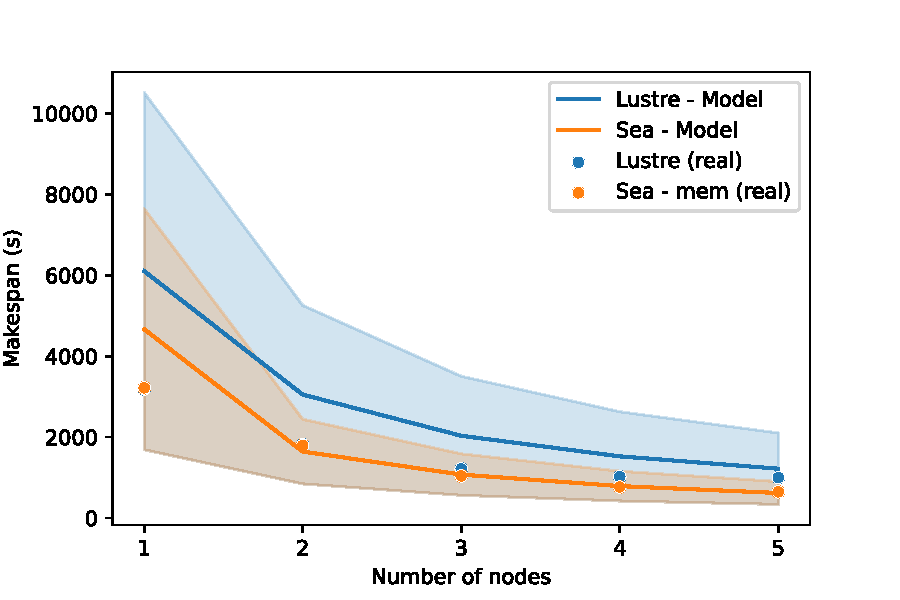
\includegraphics[width=0.8\linewidth]{figures/nodes.pdf}
            \caption{Experiment~\ref{exp:nodes}: Nodes}
            \label{fig:nodes}
        \end{subfigure}%
        \begin{subfigure}{0.5\textwidth}
            \centering
            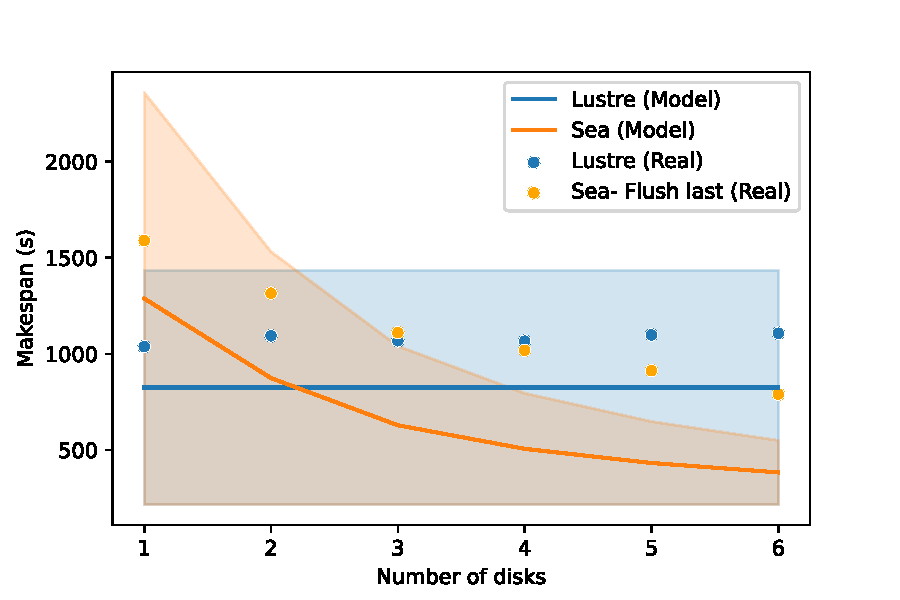
\includegraphics[width=0.8\linewidth]{figures/disks.pdf}
            \caption{Experiment~\ref{exp:disks}: Disks}
            \label{fig:disks}
        \end{subfigure}
        \begin{subfigure}{0.5\textwidth}
            \centering
            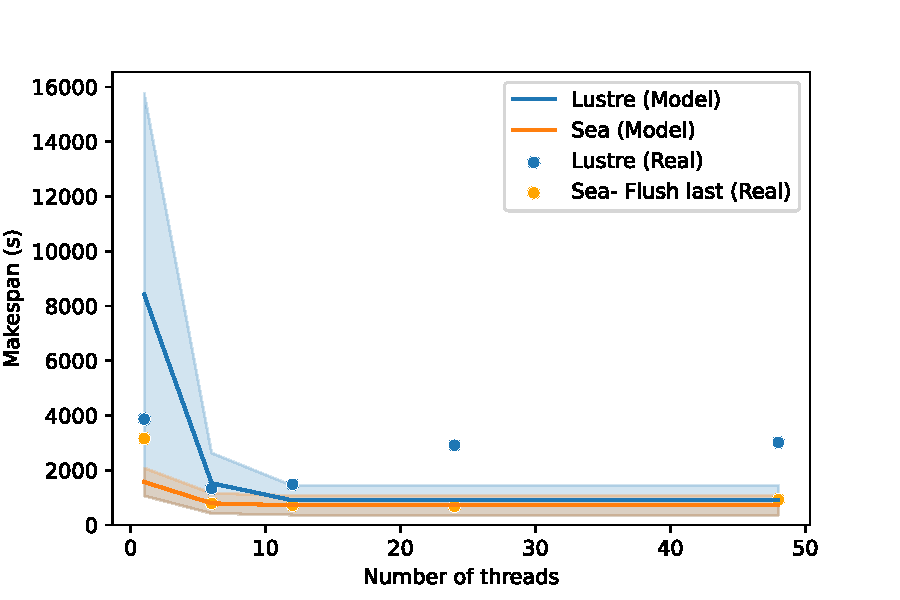
\includegraphics[width=0.8\linewidth]{figures/threads.pdf}
            \caption{Experiment~\ref{exp:threads}: Threads}
            \label{fig:threads}
        \end{subfigure}
        \begin{subfigure}{0.5\textwidth}
            \centering
            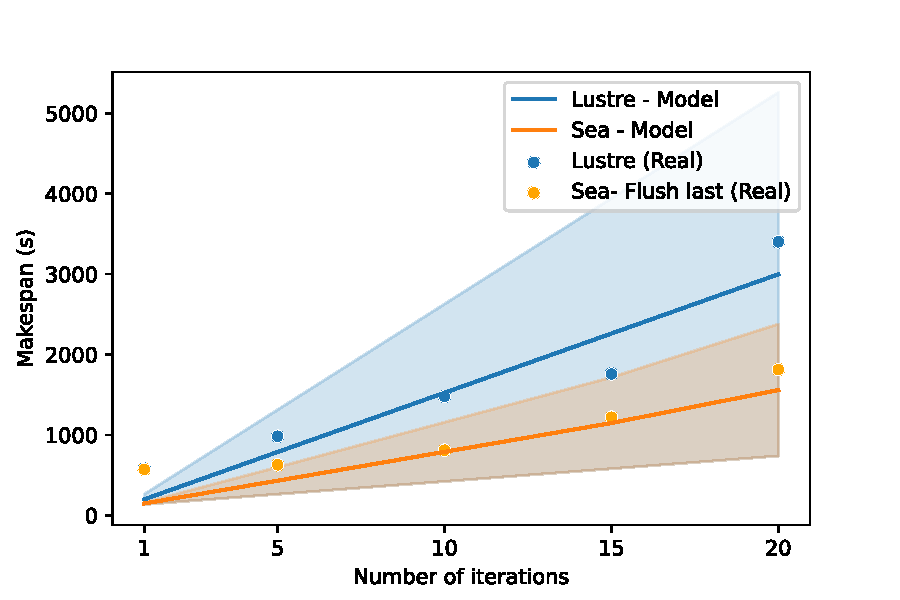
\includegraphics[width=0.8\linewidth]{figures/iterations.pdf}
            \caption{Experiment~\ref{exp:iterations}: Iterations}
            \label{fig:iterations}
        \end{subfigure}
        \caption{File system and model evaluation of Sea and Lustre. Shaded
        area represents makespan range, as determined by the model, with the
        lines representing the average of the bounds.}

    \label{fig:seaexp}
\end{figure}
    For the most part, the model appears to correctly encapsulate the
    performance range of Sea and Lustre, often times with the real data being
    situated at the halfway point between the min and max performance bounds.
    However, there are some notable exceptions.
    In Figure~\ref{fig:disks}, the model appears to adequately describe the
    performance of 1 and 2 disks, but the real results progressively surpass
    makespan estimates as the number of disks increases further. Model estimates
    for Lustre, however, encapsulate the results obtained. Interestingly
    enough, curve of the mid point line seems to parallel that of the results.

    Model estimates appear to be inaccurate to for Experiment~\ref{exp:threads}, as seen in
    Figure~\ref{fig:threads}. For 1 and 6 threads, the results occur within
    the bounds of the model, however, at 12 threads, the real results start
    to exceed model estimates and then plateau at somewhere around 24 threads.

    In Figure~\ref{fig:iterations}, although model and results appear to
    generally be in accordance with each other, the model captures neither
    Sea's or Lustre's actual makespan. Furthermore, it is unclear from the
    results if the trend is actually linear.

    The greatest overall speedup occurred in Experiment~\ref{exp:threads} at 24 threads. In 
    this experiment, Sea was 4.3~x faster than the same conditions on Lustre.
    The second highest speedup also occurred in Experiment~\ref{exp:threads}, when using 48
    threads. Sea was approximately 3.3~x faster than its Lustre counterpart.
    Otherwise, the maximum speedup obtained with Sea was 1.5~x in Experiment~\ref{exp:nodes},
    1.4~x in Experiment~\ref{exp:disks} and 1.9~x in Experiment~\ref{exp:iterations}.

    In general, Sea's performance was not worse than that of Lustre's. The only
    time there was a noticeable decrease in performance occurred in Experiment~\ref{exp:disks}
    when the number of disks used was below 3. This is a result of there being
    a greater contention on local storage with a reduced number of disks. While
    the local storage device bandwidths exceed that of Lustre \gls{ost}s (Table~\ref{table:fs}), Lustre has significantly more disks available that the overall
    attainable bandwidth is greater than that of local storage. Furthermore, 
    the network bandwidth to Lustre is also superior to the combined local
    storage bandwidth.

    \section{Discussion}\label{discussion}

    Overall, our results show that Sea performs better than Lustre when there is
    increased contention on Lustre as compared to the local storage devices. We
    expect that contention to Lustre will be significantly greater on a 
    production cluster where many users are accessing Lustre at the same time.
    As this may be the case, we might even expect Sea to outperform Lustre when
    processing data in a sequential application. However, as can be seen in
    Figure~\ref{fig:disks}, when local storage contention is greater than that
    of Lustre's, it is not recommended to use Sea. To circumvent this issue
    such that a user would not need prior knowledge on file system usage trends
    before deciding whether or not to use Sea, Sea could periodically benchmark
    the different file systems to ensure that the file is written to the most
    appropriate location.

    The model accuracy generally appeared to adequately capture Sea and Lustre
    performance trends, however, failed in some cases.
    For Figure~\ref{fig:disks}, the inaccuracy of the model might be due to poor
    SSD bandwidth estimation as the trend appears to be similar to real results.
    
    The model predictions for Experiment~\ref{exp:threads} may be off for Lustre as a result
    of metadata contention. Whereas we have many \gls{ost}s and data nodes for
    data storage, we only have a single disk dedicated to metadata storage (\gls{mdt}).
    This normally would not have been a problem, except the \gls{mds} can only support
    32 threads at a time and at 8 concurrent threads per node, we reach this limit.
    The model, at the moment, does not consider latency for metadata requests, and 
    therefore, is unable to properly describe this behaviour.

    Similarly to Lustre, model prediction error for Sea in Experiment~\ref{exp:threads}
    may arise from unaccounted for factors, such as compute time, which would otherwise
    be insignificant with a greater number of threads. What is interesting is perhaps
    the closeness in proximity that Sea's makespan is to Lustre's at a single thread.
    There may be cache effects at play here as well, in the sense that 
    \note{make stacked chart here..also wait for updated results}













    \chapter{Conclusions and Future work}

\end{document}
